\documentclass[10pt,conference]{IEEEtran}
%\documentclass[a4paper,12pt]{article}

\usepackage{cite,latexsym,times,epsf,amsmath,amssymb,amsfonts,graphicx}
\usepackage{epstopdf}
\usepackage{graphicx}
\usepackage{subfigure}
\usepackage{multirow}
\usepackage{algorithmic}
\usepackage{algorithm}
\usepackage{verbatim}
\renewcommand{\algorithmicrequire}{\textbf{Input:}}
\renewcommand{\algorithmicensure}{\textbf{Output:}}
\renewcommand{\baselinestretch}{0.95}

\begin{document}
\title{Leveraging Diverse Propagation and Context for Multi-Modal Vehicular Applications}
\author{Pengfei Cui, Hui Liu, Jialin He, Onur Altintas, Rama Vuyyuru, \\
Dinesh Rajan, and Joseph Camp\\ 
%Department of Electrical Engineering,\\ Southern Methodist University (SMU), Dallas, TX \\
%\{camp\}@smu.edu  \\
}


%\documentclass[10pt]{article}

%\usepackage{xkvltxp}
%\usepackage{fixme}


\maketitle


\begin{abstract} 

Vehicular wireless channels have a high degree of variability, presenting a
challenge for vehicles and infrastructure to remain connected. The emergence of
the white space bands for data usage enables increased flexibility for vehicular
networks with distinct propagation characteristics across frequency bands from
450 MHz to 6 GHz. Since wireless propagation largely depends on the environment
in operation, a historical understanding of the frequency bands' performance in
a given context, could speed multi-band selection as vehicles transition across
diverse scenarios.  In this paper, we leverage knowledge of in-situ operation
across frequency bands with real-time measurements of the activity level to 
select the optimal band for the particular application in use.  To do so, we
perform a number of experiments in typical vehicular topologies.  With a
model based on a Decision Tree and an in-situ training set, we can predict
the throughput on a free channel. 
We can then consider the activity level per band to compute the resulting performance 
one could expect on context information to guide protocol. In the field, we 
exploit the propagation differences experienced per band to show that training on a repeatable 
route can yield vast performance improvements from prior schemes.  We show that minimal  
amounts of training can provide such improvements and that a simple scheme that can allow
multiband adaptation gains when there is insufficient levels of training.


%Probably at this time we could not employ the bus doing the experiments.

%Unused spectrum whitespaces in the currently underutilized analog TV bands are able to exploit for future wireless networks. There are potential room for performance improvement of wireless communication in throughput, power consumption and link fairness extending wireless to these bands. Previous methods are focused on channel adaptation across multiple channels in one band without considering the propogation and other characters among different bands. In this work, we employ the propogation difference for performance prediction of multiband adaptation. To identify the crowded level,we involve an activity level of networks based on the statistics information during a time slot to make the prediction more accuracy. The amount of context information required for multiband adaptation and the influerence of window size for activity level are evaluated in this paper. We conduct indoor and in-field experiments to validate our method. The experimental results demonstrate that our method is able to achieve as ... 


\end{abstract}





%\section{Contributions}
\label{sec:introduction}


The main contributions of our work are as follows:
\begin{itemize}

\item Understand the role of propagation on multiband information via the use of context information.
\item Evaluating the amount of training necessary for gains in multiband adaptation.
\item Leverage path loss estimation in a particular environment when there is insufficient contextual training
to produce gains.
\item Verify the framework through emulated, indoor, and in-field experimental trials.
\end{itemize}






\section{Introduction}
\label{sec:introduction}


%Background
Drivers can benefit from a wide array of vehicular applications ranging from real-time traffic monitoring and
safety applications to {\it infotainment} applications spanning news, weather, audio, or video streams.  
However, the continuous use of such applications is limited due to the challenge of transmitting over 
highly-dynamic vehicular wireless channels. In such networks, the increasing availability of different 
frequency bands with correspondingly diverse propagation characteristics could allow flexibility and 
robustness of vehicular links. Even with such spectral flexibility, links are extremely tenuous, 
demanding nearly instantaneous decisions in order to remain connected and motivating an algorithm that
can find the appropriate frequency band quickly and according to the current application.

Prior work has considered a number of challenges in
leveraging the digital white space frequencies including spectrum sensing, frequency-agile operation,
geolocation, solving stringent spectral mask requirements, and providing reliable service
in unlicensed and dynamically changing spectrum along with corresponding 
protocols~\cite{shellhammer2009technical}. In particular, there has recently been an acceleration
in spectrum sensing work~\cite{rayanchu2011fluid, kim1996pulse,cabric2004implementation}. Based on 
these works, protocols have been built for multi-channel and/or multi-band wireless operation~\cite{MOAR,
raychaudhuri2003spectrum,sabharwal2007opportunistic}.  Other works have presented a method for searching the most efficient 
transmission channel~\cite{mo2005comparison}, discovering channel information from limited 
measurements~\cite{rayanchu2011fluid, sabharwal2007opportunistic}, and estimating 
channel quality through limit information~\cite{MOAR}. 

While these works have considered spectral activity and developing protocols and algorithms to 
find spectral holes, less of a focus has been on coupling such information with the propagation 
changes that frequency differences of hundreds of MHz to GHz could have on the band decision.  
Moreover, it is well known that propagation greatly depends on the environment in 
operation~\cite{rappaport}.  Thus, 
knowledge of the environment in operation could allow the relationship between received power 
differences across multiple frequency bands to have much greater accuracy.  In this paper, 
we present a multi-band adaptation protocol which leverage in-situ wireless propagation 
measurements and level of per-band activity with machine learning techniques that make a 
band choice according to application-specific performance metrics. To do so, we use an
off-the-shelf platform that allows direct experimentation across four different wireless
frequency bands simultaneously from 450 MHz to 5.8 GHz while maintaining the same physical
and media access layers.

%, it is hard to get a predict SNR just from the pathloss equation. To predict the SNR, a context-aware method is involved in this paper and combine with other methods to predict parameters for multiband adaptation.

%Activity level
%There are other factors will influence the wireless performance in different bands. One factor we are focusing on is the crowd level in different bands. Tons of wireless devices have been used all the world and completed with each other. 
%A concept \emph{activity level} which is the percentage of time the interference nodes occupied is included in this framework to qualify the crowd level. 
%In our framework we analyze the effect of crowd level using \emph{activity level} to estimate the available transmission time for a dominant factor. As a result, we formulate the \emph{Multi-band} adaptation problem to the throughput calculated from known Signal Strength and received packages. We verified the protocol on emulated, indoor and in field experiments to experimentally evaluate our approach. 

%Framwork
%The process of our framework is used to predict the performance involve context-aware information of multi bands. The context-aware information is from ideal channel(Emulator), indoor, in-field experiments. Support Vector Machine(SVM) is employed to connect the dynamic information to the context-aware information.  
%We evaluate our methods by indoor and in field experiments across 4 bands(700MHz, 900MHz, 2.4GHz, 5.8GHz), and show that in certain scenarios our approach can 
%predict the SNR more accuracy than pathloss equation and 
%Through the framework, the performance can be improved by fixme employing multi-band comparing to single wireless band.


%Problem formulation
%To get the two parameters for the performance estimation, both theoretical and context-aware methods are involved in this paper. Based on these parameters and other fixed factors according to specific environment, such as channel type, path-loss exponent and speed of wireless nodes, we are approaching to the basic problem of multi-band adaptation. 
%The basic problem of interest is as follows: \emph{Given the information of one band, get the information of other bands.}
%To solve the problem, 
%we first build a \emph{Ideal Channel Performance Context-Aware database} through the measured data from channel emulator across a wide range of different scenarios. 
%Then, based on the database and the parameters, a tunable threshold connect the \emph{Signal Strength} and the performance of different bands.

%Wireless channels are classed to different types based on the speed, propogation, noise ando so on. A simplistic characterization of channel type example could be a vehicular A in this paper. The basic problem of interest is as follows: \emph{given the channel type and Signal Strength, find the wireless band that achieves the highest throughput.}
%To solve the problem, we first build a \emph{Ideal Channel Look-Up Table} through the measured data from channel emulator across a wide range of different scenarios. Based on this , an ideal throughput for particular signal strength without noise and interference can be connected. The protocol also holds a tunable threshold parameter that determines when the \emph{Signal Strength} is different enough from others.



%Contributions  fixme
The main contributions of our work are as follows:
\begin{itemize}
\item We first formulate the problem of selecting the optimal 
frequency band according to diverse application performance metrics
to be used in the following multiband algorithms.
\item We consider three different algorithms for comparison.  First, we consider a scheme
in which the throughput is achieved on an emulated channel (historical information) for
the current received signal level. We then adjust the predicted best band choice according to the current activity
level (real-time information). 
Second, we consider an approach based on machine learning which
considers prior throughput for a given received signal and activity level
combination.  
Third, we include user location in addition to both the emulated channel and machine learning in addition to the received signal and activity level.
%Third, we consider a second machine learning approach which considers user
%location in addition to the received signal and activity level.
\item We perform V-2-\it{Base Station} experiments to evaluate each algorithm on a repeatable pattern that
%spans multiple environment types (campus, residential, and suburban) with various activity
spans in-field environment with various activity
levels and propagation characteristics within the regions. 
\end{itemize}


%\item We define an \emph{Activity Level} and enroll the concept to dynamic throughput prediction framework. The \emph{Activity Level} can describe the channel interference in time domain.
%\item We propose a simple framework that provides a way to compare the throughput across 4 different bands. Prediction the throughput across multi-band is the precondition to select a band for transmission.  
%\item We build the Look-up Table across different bands, channel models. The LUT refer to the ideal status of the channels across multi bands. It bring benifet for the work in the future.
%We experimentally analyze our framework with simulation and in-field experiments on off-the-shelf hardware platform. The platform is Gateworks 2358 board with 802.11-based radios in different frequency bands. All the radios have a physical layer based on the IEEE 802.11 a/g standard and other sensors for data collection.

The remainder of this paper is organized as follows. In Section II, we present the multiband adaptation problem and proposed algorithms. Section III discusses experimental evaluation of the multiband algorithms. We present related work in Section IV. A summary and discussion of future work is included in Section V.

%Chris: Should we remove the V_2_V experiments in the paper?

\section{Multi-band Adaptation Model}
\label{sec:model}
In this section, we introduce the pathloss and explain the potential gain of multiband adaptation in theory. The path loss shows a generally increasing trend with distance from the base,and related to the wavelength the decibel path loss can be presented as:\cite{erceg1999empirically}

\begin{equation}
PL=20log_{10}(4\pi d_0/\lambda)+10\gamma log_{10}(d/d_0)+s
\end{equation}

In an ideal channel, if the received signal is the same among all the bands, the performance should be the same. It is a reasonable assumption verified by experiments on the emulator. The performance across different bands in different received signal shows as: {fixme insert throughput vs rssi in bypass}

And also due to the limitation of FCC, the transmitting power of an Access Point is restricted. In the limited Acess range, the path loss of different bands are varying according to their wavelength. Without considering other factors, the difference of received signal makes the performance vary in different bands. Then, for a location, there is room to improve the performance in switching band.

Another problem for wireless communication is the utility level of a channel. Most of the wifi devices are working in 2.4GHz and 5GHz as 802.11 standard. 
Our method is to employ accumulate information in a time slot to quantify the channel state. The difference in crowd level of wireless channel also provide room for performance improvement in switching band.  
%In this section, we exploit channel dynamic and accumulate information in contextual data and develop band adaptation frame for dynamic environments.Through the proposed framework, we improve the throughput of a pair of multi-radio nodes according the given context. While in this paper we focus on the application to band adaptation to show gains, the framwork has other possible applications to transmission parameter adaptation based on context information. 


\subsection{Problem Formulation}
\label{subsec:problem}
The objective of this work is to introduce a way to predict the performance of multi-bands based on limited information of a single band. 
One step is to demonstrate the improvements in performance by leveraging information of ideal channels to make band adapatation decisions. 
As noted before, the context information we consider is the channel type, measured received signal strength, received bytes, background noise and channel interference. 
The channel type indicates the propagation and fading characteristics between the transmitter and receiver. Many factors(e.g., multi-path, path loss, and shadowing) have a substantial influence on the characteristics of the channel type.FIXME{citation of Hui paper} However, in this paper, we assume the channel type to be a static channel type across all the wireless bands. We use the defination of ITU channels, which are widely accepted as representative channel types for urban dan suburban settings \cite{recommendation19971225}. Moreover, noise and interference gradually changes in the field. The gradually changing process makes it possible to seperate the noise, and even the interference from time varying experiments. 
%The objective of this work is to demonstrate the improvements in performance by leveraging information of ideal channels to make band adapatation decisions. As noted before, the context information we consider is the channel type, measured received signal strength, received bytes, background noise and channel interference. The channel type indicates the propagation and fading characteristics between the transmitter and receiver. Many factors(e.g., multi-path, path loss, and shadowing) have a substantial influence on the characteristics of the channel type.FIXME{citation of Hui paper} However, in this paper, we assume the channel type to be a static channel type across all the wireless bands. We use the defination of ITU channels, which are widely accepted as representative channel types for urban dan suburban settings \cite{recommendation19971225}. Moreover, noise and interference gradually changes in the field. The gradually changing process makes it possible to seperate the noise, and even the interference from time varying experiments. 

So far, there is no work has done for such multi-band adaptation. 
Some multi-channel adaptation and rate adaptation scenarios are focus on \emph{Dynamic Channel State} as represented by \cite{cordeiro2007c,MOAR}:. 

\begin{equation}
f(SNR,Context-Aware\, Info) \rightarrow Channel
\end{equation}

which assumes that the performance is only related to the channel dynamic information. However, in our approach, we consider the intereference of channel state as a factor of statistics of time. The intereference factor gradually changing process makes the statistics have an embedded temporal correlation. We adapt the transmission band for each scenario based on the contextual information and the temporal correlation. 


In this paper, we involve a factor \emph{Activity Level} to the framework. For our case, the multi-band adaptation can be simply represented as:

\begin{equation}
f(SNR,Activity\, Level,Context-Aware\, Info) \rightarrow Band
\end{equation}

The new factor \emph{Activity \, Level} is defined as a statistics of band occupacied time ratio. Through the temporal correlation parameter, the prediction of the performance could match in-field system better than only consider the dynamic channel state.

\begin{figure}
\centering
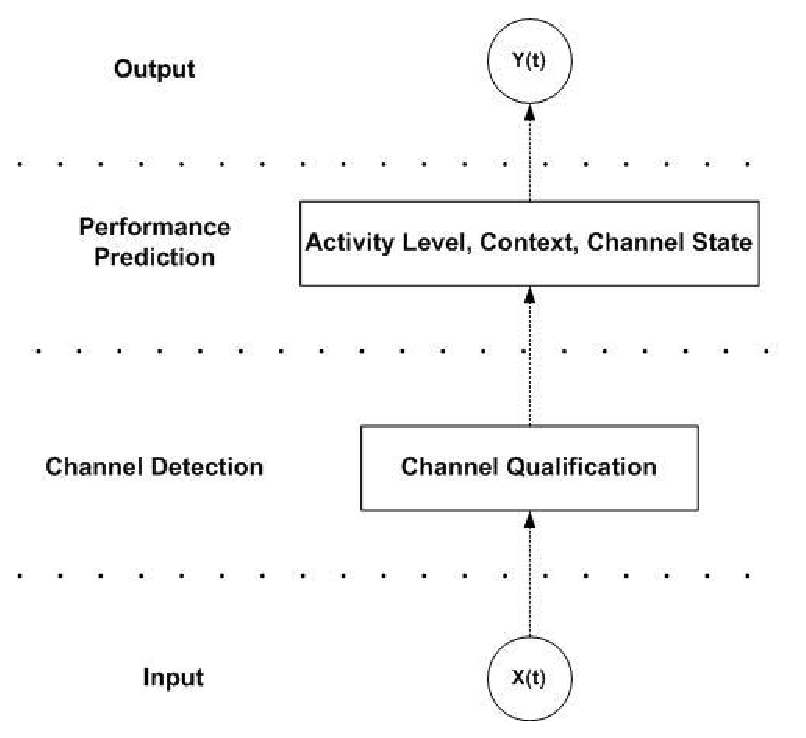
\includegraphics[width=85mm]{figure/multiband_framework}
\caption{Multiband framework.}
\label{fig:multiframe}
\end{figure}





\subsection{Context-Aware Information}

%1,what is context info


Contexts, which defines various operating situations. Depending on a context, the wireless device changes its operational 
behavior in accordance with a defined profile, when a context parameter changes \cite{phillips2004wireless}. Context is a database include the knowledge the system stored or learned from the experiments or activities. Based on tons of measurement under different parameters, a relationship between performance and system parameters can be created. In our band adaptation framework, the collected contextual information is the input to the multi-band adaptaion model. In the ideal channel context information, for each given set of bands, SNR, the context table can represent ideal throughput for each bands. 

%2,how others use the info Fixme
Context-aware information is the experience of a transmitor receiver pair. The performance of a system in the past can help transmiter to find the optimal rate/band based on the parameter collected by the receiver. Such as in FARA algroithm, the receiver uses an SNR characterization table that lists the minimum SNR required for a particular combination of modulation and coding rate\cite{rahul2009frequency}. 
Context-Aware information show a way to map the channel states to the performance.
%3,how we use the info

In our band adaptation framework, the collected contextual information is the input to the multi-band adaptaion model. In the ideal channel context information, for each given set of bands, SNR, the context table can represent ideal throughput for each bands. 
%4,Difference
The ideal throughput is part of the input information for our model to get the final decision of band adaptaion.  It is the middle state of our model to get the prediction of the performance. 







\subsection{Dyanmic and Correlation Info}

%1,How to evaluate channel
SNR is the most widely used parameter to qualify channel state \cite{rahul2009frequency}. SNR is a parameter can represent the channel state dynamicly.
%2,SNR
Many hardware manufactures already perform the SNR/Received signal strength detection character as part of the hardware specification \cite{edalat2006measured}. Mapping the SNR value to the context information is widely used in cognitive radio for estimation \cite{laneman2000energy,laneman2001efficient}. In this paper, we employ SNR as one of the factors to estimate the performance.

%3,Loss based
Moreover, there are also other factors are involved to qualify the channel. 
FARA tracks the the number of active clients, then update the nexthop table for transmission\cite{rahul2009frequency}.
The statistics of collisions and link errors also could be considered as channel qualification factors \cite{pang2005rate}.
We also define the activity level as a fctor of the channel accumulate in time domain to estimate the wireless performance.
%4,The definitation of the activity level
In our work, the definition of activity can be represented by:


\begin{equation}
\label{equation:Activity Level}
Activity\,Level = \frac{(Total\, Packets)-(Connection\, Packets)}{Average\, Rate*Duration}
\end{equation}

The activity level is a ratio that occupied by the intereference transmiter during a period. Total packets is the amount of packets received in one band during the period. The connection packets is the amount of packets accepted by particular transmitter and receiver pair. We assume all the nodes have a common rate or could be averaged to a transmission rate. The activity level represent the free time ratio can be used by the focused transmitter and receiver transmission. The interference nodes transmission has correlation between continuous periods, so the previous channel state can be used to estimate the current channel states.

%5,How we use these information

\subsection{Channel State and Performance Prediction}

The multi-band adaptation is receiver driven: the receiver node estimate the channel state, coputes the optimal choice of band across all the band, and feeds it back to the sender. The process of estimation is described as follows.

Let set $S$ denote the n-tuple of the number of bands can be selected. In the numerical results, we consider the set $S$ for white space and current common wifi wireless bands. $S={m}$, where $m \in \{\mbox{\it 700MHz},\mbox{\it 900MHz},\mbox{\it 2.4GHz},\mbox{\it 5.8GHz}\}$ represents the band that is selected. Let C represent the possible context information from previous measurements for a particular band with given parameters.

In this paper, the optimization metric of interest is the measured throughpt G. The optimization problem is stated as follows: Givern a particular context ${c\in C}$, select the optimal $s^* \in S$ that maximizes the throughput, $G_{th}$ , wehere the $T_{ideal}$ is the throughput from the ideal channel conditions in emulator. Formally, the problem is posed as follows:


\begin{eqnarray}
\max_{s \in S}& G_{th}& = (1-\mbox{\it Activity Level})*R_{th} \label{eq:throughput_optimization} \\
		\mbox{\it given} & & \mbox{\it Signal Strength}, \mbox{\it velocity}, \mbox{\it channel type} \nonumber
		\end{eqnarray}

where Activity Level is a ratio as notified represent the time during one period occupied by other nodes. The optimization problem is solved using a look-up table has the relationship of SNR and throughput mapping generated from experiments in ideal channel states, in our case collecting the data on channel emulator.  


Different variations of \ref{eq:throughput_optimization} we consider include: (\emph{i}) We map the context-aware information to find the maximize throughput across the bands in vehicular channel model.(\emph{ii}) We verify our protocol through in-field experiments data collecting on campus, so we have an assumption that the velocity of the nodes is limited for a low speed. The corresponding maximal throughput,$G^*$, serves as an upper bound to the performance that can be achieved by multi-band adaptation. This upper bound is computed off-line from the experiments data on emulator as the performance in ideal channel and all transmission time is free to use for the focused transmission pair.

%Fixme{Figure}





To be clear, we list the steps to estimate the throughput for multi-band as follow:

\begin{itemize}
\item \emph{Step 1} Collect context data on emulator for different scenarios (Bands, Channel type, SNR, Velocity) to find the ideal state or the upper bound of the performance for one band.
\item \emph{Step 2} Detect the SNR to qualify the wireless channel dynamicly, map the SNR to the context-aware information in \emph{Step 1} finding the upper bound of for the current wireless channel state.  
\item \emph{Step 3} Compute the \emph{Activity Level} according to the statistic information, then re-calculate the estimate throughput including the \emph{Activity Level}.
\item \emph{Step 4} Compare the estimate throughput across all the bands and make the best choice among the available bands.
\end{itemize}

Through these steps, the transmitter and receiver pair updates the channel state and put the best band in working.





		%Fixme




\section{Experimental Analysis for Prediction Algorithms}
\label{sec:experiment design}

%In this section, the experiments on emulated channel, and in-field for estimation and evaluation are introduced. The equipments ,methods and experiments environments are involved as part of the experiments design.
%for repeatability and control to directly compare and evaluate different bands performance and design in-field experiments to have the data for training and testing on campus. 
%The experimental results are used for the framework and the framework verification. 
%dicate that the application of multi-band adaptation can enchance the performance of a transmitter and receiver pair. 

As discussed in Section 3, the algorithms are fit for different scenarios. To study the difference of the algorithms and find the parameter patterns of these schemes, we have developed indoor and in-field experiments 
on widely used off-the-shelf wireless platform.
%Testbed and emulator Platform
To ensure the results are broadly applicable across wireless device, we employ widely accepted 802.11 testbed. Gateworks 2358 with Ubiquiti XR serial radios,XR9 (900MHz), XR2 (2.4GHz),XR5 (5.8GHz), SmartBridges 450MHz Radio, open source Linux based software to make the experiment plan \cite{Gateworks,Ubnt,Openwrt}. 
Another instrument involve in the experiments is channel emulator,
Azimuth ACE-MX, which is used for channel emulation, allowing controllable propagation and fading characteristics with a broad range of industry-standard models in 450MHz-2700MHz, 3300MHz-3800MHz, 4900MHz-5900MHz \cite{AzimuthACE}. 


%context information experiments
\subsection{Data of Hardware Performance Collection}
\label{subsec:ichannel}
To get data for \emph{SNR based Throughput Look up Algorithm}, we use an experimental setup where two wireless nodes communicate across emulated channels generated by Azimuth ACE-MX channel emulator. 
The channel emulator can create repeatable channels for collecting RSSI and throughput data.
%The channel emulator can create repeatable channels for testing each wireless band to measure the performance for a given wireless context. 

\begin{figure}
\centering
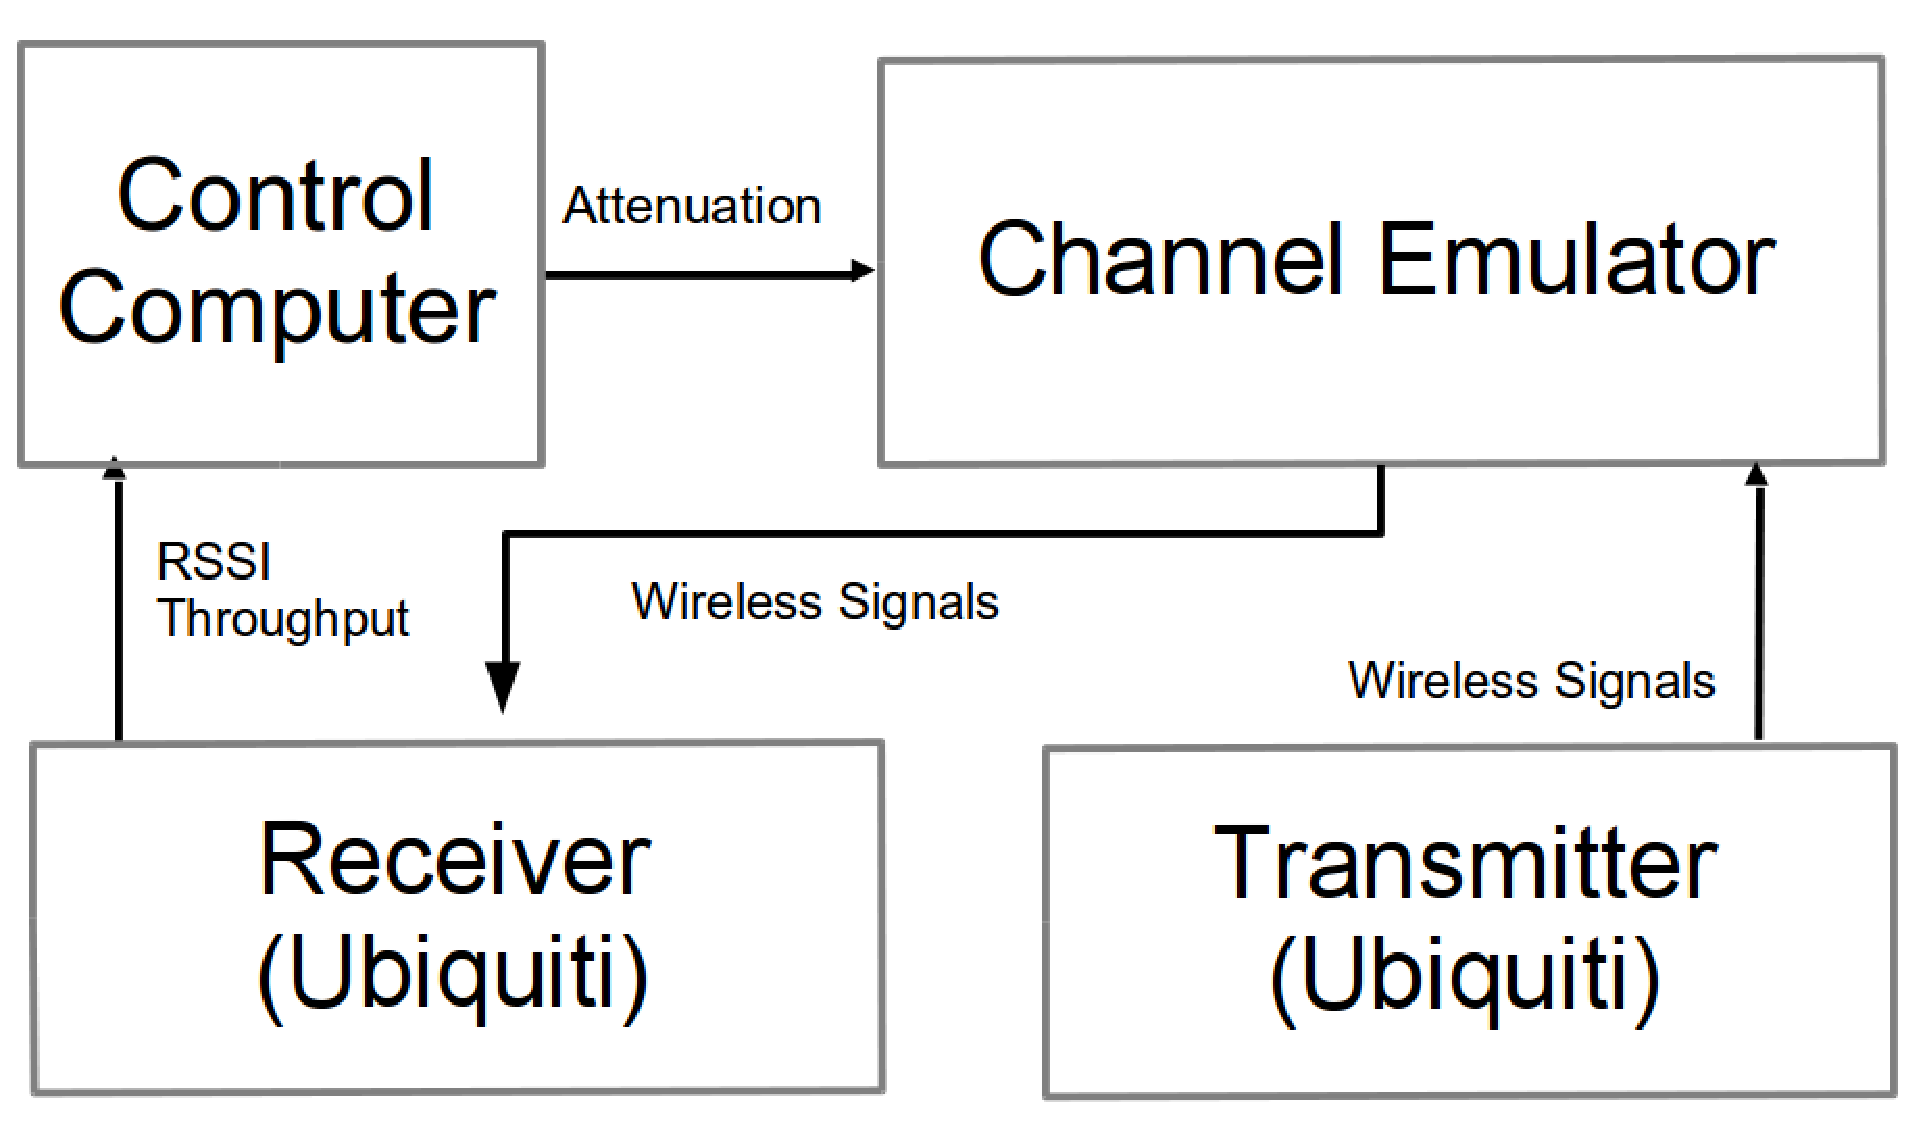
\includegraphics[width=85mm]{figure/emulator2}
\caption{Hardware Performance Experiment Setup}
\label{fig:in-door experiment}
\end{figure}

For this scenario, in a given band, we repeat the experiments under different configuration to get the throughput information across multiple bands in an ideal channel environment with different RSSI as shown in Figure \ref{fig:in-door experiment}.

Also, according to the emulator experiment data, the throughput performance could be normalized to remove the discrepancy of the radios for comparison across all the bands fairly. 
%the band adptation algorithm will extract the relationship between the contextual information and the target band.


%\subsection{Signal Level Context-aware information}
%There are two parts of this scenario in different environments, indoor and in-field. The experiments are done in the lab and on campus. We analyze the influence of the information amount for the prediction. 
\subsection{Experimental Design for In-field Data Collection}
\label{subsec:insitu}
In the in-field experiments two Gateworks nodes with 4 radios are installed on two cars, one works as receiver, another works as transmitter moving around a public park as shown in Figure \ref{fig:infield}.

\begin{figure}
\centering
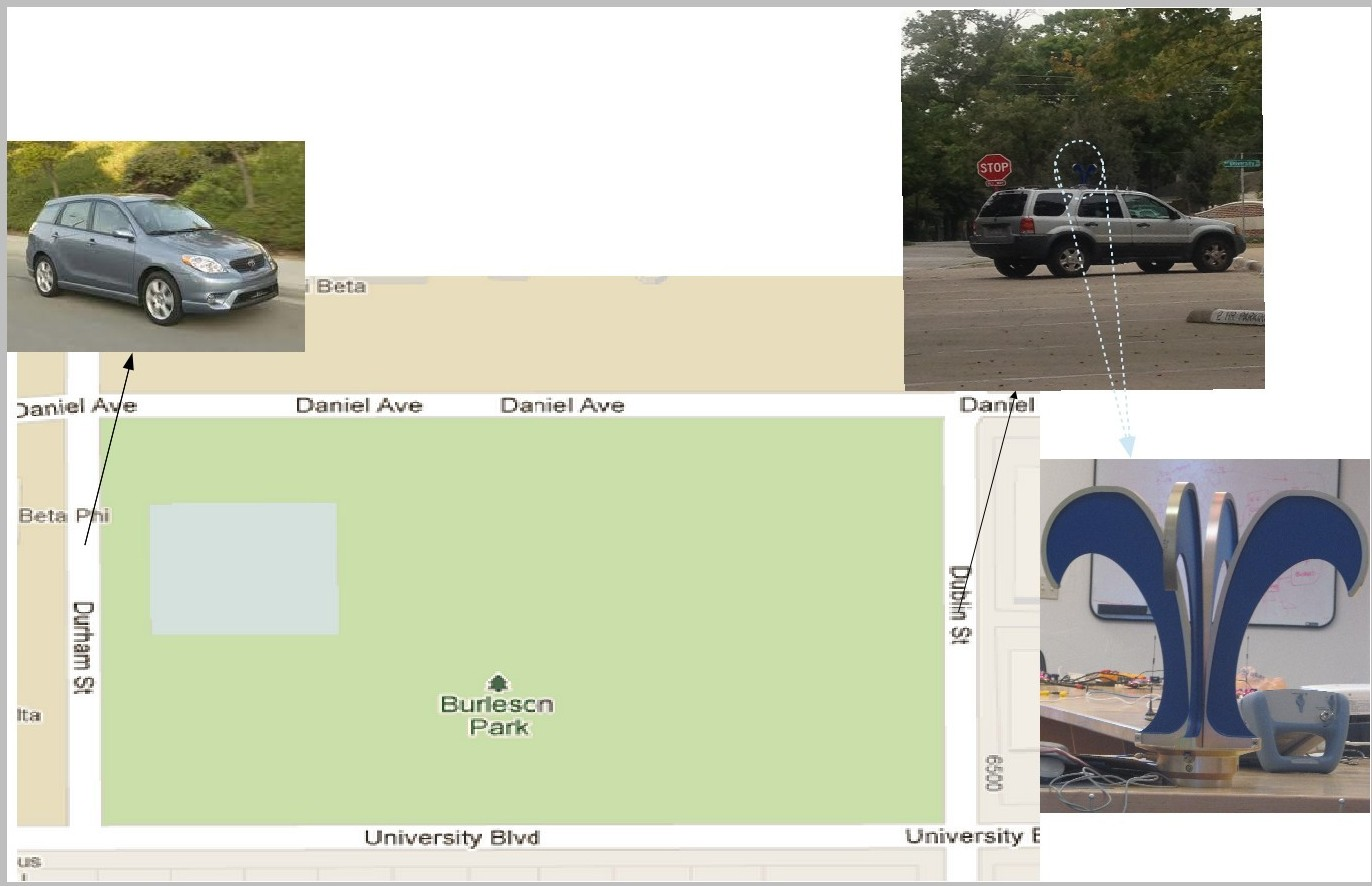
\includegraphics[width=85mm]{figure/infield}
\caption{In-field Experiment Setup}
\label{fig:infield}
\end{figure}

One of the car park in a fixed location work as a receiver, then another car work as a transmitter drive around the park for several loops to get the data with parameters. 
In receiver node, all the packets can be received are dumped for calculation of the parameters for algorithms. 

As shown in in Figure \ref{fig:infield}, we use an multi-band antenna work with an spectrum analyzer to detect the signal in the air. All the activity can be seen on the data get from spectrum analyzer.
Also, all the 802.11 packets are dumped by Tcpdump installed on Gateworks wireless nodes \cite{jacobson1989tcpdump}. Then based on the time stamps, 802.11 packets can be recognized and only non 802.11 interference will be counted from the spectrum analyzer data in data processing.  
%Input spectrum analyzer process figure, explain

\begin{figure}
\centering
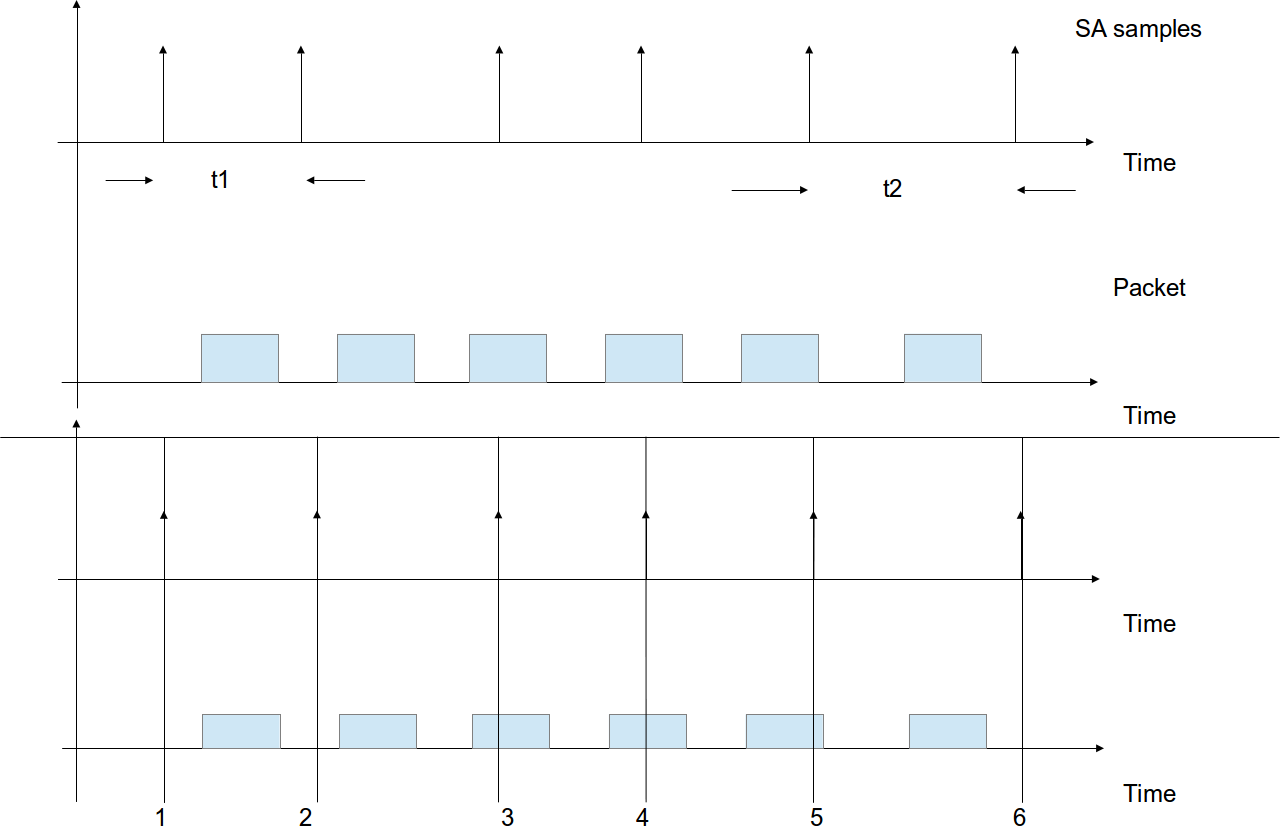
\includegraphics[width=85mm]{figure/sa_process}
\caption{Spectrum Analyzer Data Processing}
\label{fig:sa_process}
\end{figure}

Figure \ref{fig:sa_process} shows the process to get the \emph{Non 802.11 Interference Signal}. The spectrum analyzer (SA) samples match the dumped 802.11 packets are deleted, such as No. 3, No.4 and No.5. Then, the samples will not mix with the 802.11 packets and be counted twice in algorithms.


The in-field data is processed offline. As discussed in \ref{subsec:ideal channel}, the throughput was normalized based on the emulator experiment to balance the diversity of hardware performance. Then, data from different devices and software is synchronized based on the GPS/System time stamps.


%\subsubsection{Activity Level Measure} 
%Madwifi is the driver widely embedded in Linux based wireless operating system, as in OpenWRT \cite{Madwifi,Openwrt}. Madwifi provide an interface for sniffer to get the information of each packet.
%For the in-field scenario,
%to get the \emph{Activity Level,SNR} as the input of our algorithm, 
%we calculate from the dumped packets information. The transmitting rate and length of each packet can be captured by sniffer.%The \emph{Activity Level} is calculated by these information.

%to map the total received packets, our focused transmitter-receiver pair received packet, received signal power, background noise and interference. We use two Gateworks platform with Ubiquiti radios combining Agilent Spectrum Analyzer to collect data for our off-line analysis. We map these data synchronous through timestamp from GPS information on our testbed and the system time on the Spectrum Analyzer.

%To calculate the \emph{Activity Level}, the raw data we need is the total received packets and the focused transmitter-receiver pair received packets during a small time slot. 
%To measure the throughput and calculate the focused transmitter-receiver pair received packet(Focused RX packet) in a less than 1 second time slot, a socket program is generated for the experiments. The transmitter side could send packets in a 500ms duration, then turn off the transmission for another 500ms to meaure the interference. These raw data could be put into \ref{equation:Activity Level} calculate the activity level for the future prediction.


%in-field experiments design
%Gateworks, socket, spectrum analyzer
%\subsection{In-field Experiments}

%\subsubsection{Signal Measure}
%For the in-field experiments, the nodes has the same configuration. But we put the transmitter node and one receiver node in a location, the other receiver node on a car. In this scenario, the input of the frame work includes velocity, and all the context-aware database information and test information are collected from the receiver node on the car.

%We need the pure signal power from the transmitter to extract the ideal throughput from the context information we got from emulated channel experiments. It is impossible to get the interference during the transmitter sending period. So the transmitter is configured to turn on for a 500ms transmission to measure the throughput and the signal power(noise, interference and transmit power), and then turn off for another 500ms to measure the interference strength. 

%Fixme figure of the experiment flow

%SA utility
%The testbed could report the received strength, howerve, it could not update the value without transmission. The method we use to collect the signal strength is to record the spectrum activity through an Agilent Spectrum Analyzer. Agilent MXA N9020 Signal Analyzer could monitor a wide band spectrum and record the spectrum activity in a CSV file for a time point \cite{SA}. To get the continous record during the experiments, a MFC(Microsoft Foundation Class) dialog software is generated to control the spectrum analyzer to save the record file periodicly through Agilent I/O Command Expert\cite{MFC,AC}. We also record the signal strength on the testbed to match the record from spectrum analyzer.

%A node in a car works as the transmitter, and another node with the spectrum analyzer located in a fixed place work as the receiver. The car drive one loop on campus for a measurement of one band. During one loop, the throughput, RX packets, Focused RX packets, signal strength in transmission on and transmission off are collected. 

%Based on these collected data, the off-line data process are done with accuracy and improvement as metric to evaluate the methods.  
%


\section{Data Process}
\label{sec:experiment}

Fixme


%Detail may not useful
Parsing script
In our experiments, we are constantly collecting large amounts of data, including the received signal level, current location, velocity, and time of day. Working with the memory-limited Gateworks boards, it became necessary to implement a solution to collect large amounts of data without exhausting the available memory space on the boards. Thus, we compiled a script to parse an undetermined number of data files containing the raw data collected from the ongoing experiments. Utilizing the Perl programming language, which the Gateworks boards are capable of running, the script scans every file in a directory we specify and parses them, looking specifically for signal level, lat/long location, velocity, and time data recorded from the experiments. Upon finding this information, the script reformats the data by placing it into a .csv file. Additionally, using the location data, the script calculates the  distance between the transmitting and receiving boards and adds this information to the .csv file. Upon parsing the data, the raw experimental data files can simply be delete from memory, freeing up space for the data of subsequent experiments.

Activity monitor script
For in-situ experiments, the need became apparent to track the number of new incoming packets and compare it with the number of previously received packets. Additionally, this needed to be done for each of the four wireless radios on the board. In doing this, we identify the most efficient frequency band to transmit data. To implement this system, a script was needed to run efficiently in the background while experiments were taking place. To achieve this, we wrote a bash shell script to run directly on the board without relying on any higher level programming language that could potentially cause greater performance overhead. As a result, the script only consumes one to two percent of CPU resource. The script begins by examining the received bytes across each radio for a length of 30 seconds and placing the bytes received each second on a new line in a file. Upon the completion of the 30 second buffering time period, the next second of received bytes on each radio is read and compared with the last 30 seconds of received data. This ratio of the most recent received data to old received data is then calculated and written to four files, one for each radio, for its subsequent use in selecting which radio to transmit/receive from.


%\section{Related Work}
\label{sec:related}
%%fixme add the daparowrds
%The conventional definition of the spectrum opportunity, which is often defined as "A band of frequencies that are not being used by the primary user of that band at a particular time in a particular geographic area."\cite{kolodzy2001next}


Elecronmagnetic radio spectrum is a natural resource licensed by governments.  the Federal Communications Commission(FCC) published a report prepared by the Spectrum-Policy Task Force, discussed improving the way to manage this resource in the United States \cite{federal2002spectrum}. 

The limited resource make people find new ways to improve the effciency of the frquency resource utility. There are two methods to arrive this target. First is the underlay approach, constraints on the transmission power of second users. Second is the overlay approach, identify and exploit spatial and temporal spectrum white space by second users \cite{zhao2007survey}.
The first approaching require more support from the hardware, the second approaching can be achieved by soft-ware radios only. The frequency is not occupacied all the time in all the regions.


%ways to improve the frequency efficient



The underutilization of the electromagnetic spectrum leads to a definition of \emph{Spectrum Opportunity} as a band of frequencies assigned to a primary user, but at a particular time and specific geographic location, the band is not being utilized by that user \cite{kolodzy2001next}.



%Cognitive Radio

%fixme FCC definition
%The definition adopted by Federal Communications Commission(FCC):"Cognitive radio: A radio or system that senses its operational electromagnetic environment and can dynamically and autonomously adjust its radio operating parameters to modify system operation, such as maximize throughput, mitigate interference, facilitate interoperability, access secondary markets."
The concept of \emph{Cognitive Radio} is introduced as a novel approach for improving the utilization of the wireless spectrum and the tasks for cognitive radio is summarized in \cite{haykin2005cognitive}. The three on-line cognitive tasks include: \emph{Radio-scene analysis, Channel identification, Transmit-power control and synamic spectrum management} \cite{haykin2005cognitive}.
Underutilized terrestrial TV bands will be able to be used by wireless communication. Combine different bands to create Multi-bands/Multi-channels system is a new field of \emph{Cognitive Radio} to improve the performance of wireless systems in different
environments(e.g., as in ~\cite{MOAR}). 

%Multi-channel
A bunch of work has been done on \emph{Radio-scene analysis} and \emph{Channel identification} dating back to Simon Haykin \cite{haykin2005cognitive}.
Some work of Multi-bands/Multi-channels in
cognitive radios focus on optimize performance, such as avoiding frequency diversity \cite{rahul2009frequency}. 
In \cite{OAR} an opportunistic algorithm is intorduced to balance the cost of \emph{spectrum sensing, Channel switching} and the gain of these activities.
%fixme, add more multichannel and add pathloss exponent

%spectrum sensing

One of the most important components of the congnitive radio concept is the ability to measure, sense, learn and be aware of the parameters related to the radio channel characteristics, availability of spectrum and power, radios operating envrionment \cite{yucek2009survey}. Spectrum sensing becomes the most important component for the estabilishment of congnitive radio. \cite{yucek2009survey}. 





%Adaptation algorithms
There is a lot of recent research on the design of adaptation algorithms, both rate adaptation and \emph{band/channel} adptation of cognitive radio systems. These researches are focusing on the \emph{Spectrum sensing and Channel switching strategies}.

\textbf{Evaluation of Channel Conditions}. Channel condition is the most important component of adaptation. 
There are two classes of rate adaptation mechanisms that have been developed. 
These mechanisms are focused on rate adaptation. The first generation adaptation algorithms are loss-triggered. The adaptation algorithm based on the statistics of a previous period of transmission. 
Second generation rate adaptation schemes diagnose the cause of a loss and appropriately adjust the data rate \cite{biaz2008rate, camp2010modulation}, such as a SNR-triggered protocol. 
Our work consider both the statistics information of the previous transmission and the dynamic information in context-aware based channel qualification.

\textbf{Evaluation of Adaptation}. Most of the prior work of rate adaptation protocols has investigated the effectiveness via throughput comparison \cite{camp2010modulation}. This is the metric we also employ in the paper to evaluate the performance. Furthermore, we also evaluate the amount of context-aware information in prediction.
 
\textbf{Primary Second User}. Some other works focus on Multi-channel which bandwidth range limits in 2.4GHz \cite{MOAR} or in a continuous bandwidth considering frequency diversity \cite{rahul2009frequency}. 
Significant research on the design of channel selection algorithms has been done \cite{radunovic2011dynamic,raniwala2005architecture}. Algorithms are generated for second user to distinguish whether the channel is free or in less utility state as soon as possible \cite{cordeiro2007c}. These works indicate the way to employ limit frequency work in high efficiency. In contrast, we are trying to improve the wireless performance taking more frequency bands.

Our work is motivated by prospective white band using for TV today and exploit the comparison across all the avaiable bands in the future. It is a kind of extention of multi-channel adaptation. Our approach classifies the performance based upon combination of in-field measurents and ideal channel conditions on \emph{channel emulator}. Most of the research focus on the stopping rules of spectrum sensing \cite{sabharwal2007opportunistic, OAR}. In contrast, we use the data and framework to classify the performance across different bands based on the parameters we get from the context-aware information.
{\bf .} 


\section{Conclusion}
\label{sec:conclusion}
In this paper, we investigated the multi-band adaption to leverage the propagation and context for vehicular utility. 
We did so by first testing and comparing the performance of different approaching multi-band selection algorithms. 
In our experimental analysis, we evaluated the performance of these algorithms on Gateworks hardware platform over in-field channels. 
Experimental results demonstrate that these algorithms can fit different utility environments. The accuracy of these algorithms can be up to 60.5\%.
Since for mobile utility, energy is limited, in the future work we plan to consider the energy efficient in multi-band adaptation.



\bibliographystyle{IEEEtran}

\bibliography{multiband}

\end{document}
%This is never printed
